\documentclass[../main.tex]{subfiles}

\begin{document}
\subsection*{Appendix: Differential Equation Study Guide}

    \textbf{First Order Equations.} General Form of ODE
    \begin{align*}
    \dfrac{dy}{dx}=f(x,y)
    \end{align*}
    Initial Value Problem
    \begin{equation*}
        y'=f(x,y),\ y(x_0) = y_0
    \end{equation*}

    \textbf{Linear Equations.} General Form: 
    \begin{align*}
    y'+p(x)y=f(x)
    \end{align*}
    Integrating Factor
    \begin{align*}
         \mu(x) &= e^{\int p(x)dx}\\
          \implies & \dfrac{d}{dx}\left( \mu(x) y \right) = \mu(x) f(x)\\
    \end{align*}
General Solution
\begin{equation*}
    y=\frac{1}{\mu(x)}\left( \int \mu(x) f(x) dx + C\right)
\end{equation*}

\textbf{Homogeneous Equations.} General form
\begin{align*}
 y'=f(y/x)
\end{align*}
Substitution
\begin{equation*}
    y=zx  \implies y'=z + xz'
\end{equation*}
The result is always separable in $z$: 
    \begin{equation*}
    \dfrac{dz}{f(z)-z} = \dfrac{dx}{x}
    \end{equation*}

\textbf{Bernoulli Equations.} General Form
    \begin{align*}
y'+p(x)y=q(x)y^n
    \end{align*}
    Substitution\begin{align*}
        z = y^{1-n}
    \end{align*}
    The result is always linear in $z$:
    \begin{equation*}
     z' +(1-n)p(x) z = (1-n)q(x)
    \end{equation*}

    \textbf{Exact Equations.} General Form
    \begin{align*}
M(x,y)dx + N(x,y)dy = 0 
    \end{align*}
    Text for Exactness
    \begin{equation*}
        \dfrac{\partial M}{\partial y}=\dfrac{\partial N}{\partial x}
    \end{equation*}
    Solution
    \begin{equation*}
        \phi=C
    \end{equation*}
where
\begin{equation*}
    M=\dfrac{\partial \phi}{\partial x}\quad\text{ and }\quad N=\dfrac{\partial \phi}{\partial y}
\end{equation*}

    \textbf{Method for Solving Exact Equations. }

    \begin{enumerate}
        \item Let $\phi=\int M(x,y)dx + h(y)$
        \item Set $\dfrac{\partial \phi}{\partial y} = N(x,y)$
        \item Simplify and solve for $h(y)$
        \item  Substitute the result for $h(y)$ in the expression for $\phi$ from step 1 and then set $\phi=0$. This is the solution. 
    \end{enumerate}
    
    Alternatively: 
    \begin{enumerate}
        \item Let $\phi=\int N(x,y)dy + g(x)$
        \item Set $\dfrac{\partial \phi}{\partial x} = M(x,y)$
        \item Simplify and solve for $g(x)$. 
        \item Substitute the result for $g(x)$ in the expression for $\phi$ from step 1 and then set $\phi=0$. This is the solution. 
    \end{enumerate}
    
    \textbf{Integrating Factors.} Case 1. If $P(x,y)$ depends only on $x$, where
    \begin{equation*}
    P(x,y)=\dfrac{M_y-N_x}{N} \implies \mu(y) = e^{\int P(x)dx}
    \end{equation*}
    then
    \begin{equation*}
    \mu(x) M(x,y) dx + \mu(x) N(x,y) dy = 0
    \end{equation*}
    is exact.
    
    Case 2. If $Q(x,y)$ depends only on $y$, where
    \begin{equation*}
    Q(x,y)=\dfrac{N_x-M_y}{M} \implies \mu(y) = e^{\int Q(y)dy}
    \end{equation*}
    Then 
    \begin{equation*}
    \mu(y) M(x,y) dx + \mu(y)N(x,y) dy =0
    \end{equation*}
    is exact.
    
\textbf{Second Order Linear Equations} General Form of the Equation
    \begin{equation} 
    a(t)y''+b(t)y'+c(t)y=g(t) \label{eq:general}
    \end{equation}
Homogeneous
\begin{equation}
    a(t)y''+b(t)y'+c(t)y=0\label{eq:homog}
\end{equation}
Standard Form
\begin{equation}
     y''+p(t)y'+q(t)y=f(t) \label{eq:ODE}
\end{equation}

    \textbf{General Solution.} The general solution of \eqref{eq:general} or \eqref{eq:ODE} is 
    \begin{equation}
    y = C_1 y_1(t) + C_2 y_2 (t) + y_p(t)
    \end{equation}
    where $y_1(t)$ and $y_2(t)$ are linearly independent solutions of \eqref{eq:homog}.
    
    \textbf{Linear Independence and The Wronskian.} Two functions $f(x)$ and $g(x)$ are linearly dependent if there exist numbers $a$ and $b$, not both zero, such that $af(x)+bg(x)=0$ for all $x$. If $y_1$ and $y_2$ are two solutions of \eqref{eq:homog}, then Wronskian
    \begin{equation*}
    W(t) = y_1(t) y_2'(t) - y_1'(t) y_2(t)
    \end{equation*}
    and Abel's Formula
    \begin{equation*}
    W(t) = Ce^{-\int{p(t)dt}}
    \end{equation*}
    and the following are all equivalent: 
    \begin{enumerate}
    \item $\{y_1,y_2\}$ are linearly independent.
    \item $\{y_1,y_2\}$ are a fundamental set of solutions.
    \item $W(y_1, y_2)(t_0)\neq 0$ at some point $t_0$.
    \item $W(y_1,y_2)(t) \neq 0$ for all $t$.
    \end{enumerate}
    
    
    \textbf{Initial Value Problem.} The initial value problem includes two initial conditions at the same point in time, one condition on $y(t)$ and one condition on $y'(t)$. 
    \begin{equation*}
    \left\{
    \begin{array}{l}
    y''+p(t)y'+q(t)y=0\\ y(t_0)=y_0 \\ y'(t_0)=y_1
    \end{array} 
    \right.
    \end{equation*}
    The initial conditions are applied to the entire solution $y=y_h+y_p$. 
    
    \textbf{Linear Equation With Constant Coefficients.} The general form of the homogeneous equation is  
    \begin{equation}
        ay'' + by' + cy=0 \label{eq:linearhomog}
    \end{equation}
    Non-homogeneous
    \begin{equation}
        ay''+by'+cy = g(t)\label{eq:linearnonhomog}
    \end{equation}
Characteristic Equation
\begin{equation*}
    ar^2 + br + c=0
\end{equation*}
Quadratic Roots
\begin{equation}
    r=\frac{-b\pm\sqrt{b^2-4ac}}{2a}
\end{equation}
The solution of \eqref{eq:linearhomog} of Real Roots $(r_1 \neq r_2)$
\begin{equation}
    y_h = C_1 e^{r_1 t} + C_2 e^{r_2t} \label{eq:LH1}
\end{equation}
Repeated $(r_1 = r_2)$
\begin{equation}
    y_h = (C_1 + C_2 t)e^{r_1t}\label{eq:LH2}
\end{equation}
Complex $(r=\alpha\pm i\beta)$
\begin{equation}
    y_H=e^{\alpha t}(C_1 \cos \beta t + C_2 \sin \beta t) \label{eq:LH3}
\end{equation}
    The solution of \eqref{eq:linearnonhomog} is $y=y_p+y_h$ where $y_h$ is given by \eqref{eq:LH1} through \eqref{eq:LH3} and $y_p$ is found by undetermined coefficients or reduction of order.
    
    \textbf{Heuristics for Undetermined Coefficients.} Also called Trial and Error


\begin{center}
        \begin{tabular}{|l|l|}
        \hline 
        If $f(t)=$ & then guess that a particular solution $y_p=$. \\
        \hline\hline
        $P_n(t)$ & $t^s (A_0 + A_1 t + \cdots + A_n t^n)$ \\
        \hline 
        $P_n(t)e^{at}$ & $t^s (A_0 + A_1 t + \cdots + A_n t^n)e^{at}$ \\
        \hline
        $P_n(t)e^{at}\sin bt$ & $t^s e^{at} [(A_0 + A_1 t + \cdots + A_n t^n)\cos bt$ \\
        or $P_n(t)e^{at}\cos bt$ & \ \ \ \ \ $ + (A_0 + A_1 t + \cdots + A_n t^n)\sin bt]$ \\
        \hline 
        \end{tabular}
\end{center}

    
    \textbf{Method of Reduction of Order.} When solving \eqref{eq:homog}, given $y_1$, then $y_2$ can be found by solving
    \begin{equation*}
    y_1 y_2' - y_1'y_2 = Ce^{-\int p(t) dt}
    \end{equation*}
    The solution is given by 
    \begin{equation}
    y_2 = y_1\int \dfrac{e^{-\int p(x) dx} dx}{y_1(x)^2}\label{eq:ROE}
    \end{equation}
    
    \textbf{Method of Variation of Parameters.} If $y_1(t)$ and $y_2(t)$ are a fundamental set of solutions to \eqref{eq:homog} then a particular solution to \eqref{eq:ODE} is 
    \begin{equation}
    y_P (t) = -y_1(t) \int \dfrac{y_2(t) f(t)}{W(t)}dt + y_2(t) \int \dfrac{y_1(t) f(t)}{W(t)}dt 
    \end{equation}
    
    \textbf{Cauchy-Euler Equation.} For ODE
    \begin{equation}
        ax^2y''+bxy'+cy=0 \label{eq:CEODE}
    \end{equation}
    with Auxilliary Equation
    \begin{equation}
        ar(r-1)+br+c=0\label{eq:CEODEAux}
    \end{equation}
    The solutions of \eqref{eq:CEODE} depend on the roots $r_{1,2}$ of \eqref{eq:CEODEAux}. For Real Roots
    \begin{equation*}
        y = C_1x^{r_1} + C_2x^{r_2}
    \end{equation*}
    Repeated Root
    \begin{equation*}
        y = C_1 x^r + C_2 x^r \ln x
    \end{equation*}
    Complex
    \begin{equation}
        y=x^{\alpha}[C_1\cos(\beta \ln x) + C_2 \sin (\beta \ln x)] \label{eq:comprootCEODE}
    \end{equation}
    In \eqref{eq:comprootCEODE} $r_{1,2}=\alpha\pm i\beta$, where $\alpha$,$\beta\in\mathds{R}$
    
    \textbf{Series Solutions.} 
    \begin{equation}
    (x-x_0)^2y''+(x-x_0)p(x)y'+q(x)y=0 \label{eq:SS}
    \end{equation}
    If $x_0$ is a regular point of \eqref{eq:SS} then 
    \begin{equation*}
    y_1(t) = (x-x_0)^n\sum_{k=0}^{\infty}a_k(x-x_k)^k
    \end{equation*}
    At a Regular Singular Point $x_0$, the Indicial Equation
    \begin{equation}
        r^2+(p(0)-1)r + q(0)=0 \label{eq:indicial}
    \end{equation}
    First Solution
    \begin{equation*}
        y_1=(x-x_0)^{r_1}\sum_{k=0}^{\infty}a_k(x-x_k)^k
    \end{equation*}
    Where $r_1$ is the larger real root if both roots of \eqref{eq:indicial} are real or either root if the solutions are complex. 
    \clearpage

\subsection*{Appendix: Laplace Table}
        \begin{longtable}{m{0.05\textwidth}m{0.3\textwidth}  m{0.3\textwidth}m{0.2\textwidth}}
            \hline &&&\\
            \multicolumn{2}{ p{0.35\textwidth} }{ \centering \(f(t)=\mathcal{L}^{-1}{F(s)}=F(s)\) } & \multicolumn{2}{ p{0.5\textwidth} }{\centering  \(\mathcal{L}{f(t)}=F(s) \)}\\&&&\\\hline
            \[\mathcal{L}1\] & \centering \[1\] & \centering \[\frac{1}{p+a}\]& \[\text{Re }p>0\]\\
            \[\mathcal{L}2\] & \centering \[e^{-at} \] & \centering \[\frac{1}{p}\] & \[\text{Re }p>0\]\\
            \[\mathcal{L}3\] & \centering \[\sin at\] & \centering \[\frac{a}{p^2+a^2}\] & \[\text{Re }p>|\text{Im }a|\]\\
            \[\mathcal{L}4\] & \centering \[\cos at\] & \centering \[\frac{p}{p^2+a^2}\] & \[ \text{Re }p>|\text{Im }a| \]\\
            \[\mathcal{L}5\] & \centering \[t^k,k>-1\] & \centering \[\frac{k!}{p^{k+1}}\] or \[\frac{\Gamma(k+1)}{p^{k+1}}\]& \[\text{Re }p>0\]\\
            \[\mathcal{L}6\] & \centering \[t^ke^{-at},k>-1\] & \centering \[\frac{k!}{(p+a)^{k+1}}\] or \[\frac{\Gamma(k+1)}{(p+a)^{k+1}}\]& \[\text{Re }(p+a)>0\]\\
            \[\mathcal{L}7\] & \centering \[\frac{e^{-at} - e^{-bt}}{b-a}\] & \centering \[\frac{1}{(p+a)(p+b)}\] & \ \[\text{Re }(p+a)>0\] \[\text{Re }(p+b)>0\]\\
            \[\mathcal{L}8\] & \centering \[\frac{ae^{-at} - be^{-bt}}{b-a}\] & \centering \[\frac{p}{(p+a)(p+b)}\] &  \[\text{Re }(p+a)>0\] \[\text{Re }(p+b)>0\]\\
            \[\mathcal{L}9\] & \centering \[\sinh at\] & \centering \[\frac{a}{p^2-a^2}\] & \[\text{Re }p>|\text{Re }a|\]\\
            \[\mathcal{L}10\] & \centering \[\cosh at\] & \centering \[\frac{p}{p^2-a^2}\] & \[\text{Re }p>|\text{Re }a|\]\\
            \[\mathcal{L}11\] & \centering \[ t\sin at \] & \centering \[ \frac{2ap}{(p^2+a^2)^2}\] & \[\text{Re }p>|\text{Im }a|\]\\
            \[\mathcal{L}12\] & \centering \[t\cos at\] & \centering \[\frac{p^2-a^2}{(p^2+a^2)^2}\] & \[\text{Re }p>|\text{Im }a|\]\\
            \[\mathcal{L}13\] & \centering \[e^{-at}\sin bt\] & \centering \[\frac{b}{(p+a)^2+b^2}\] & \[\text{Re }(p+a)\]\[>|\text{Im }b|\]\\
            \[\mathcal{L}14\] & \centering \[e^{-at}\cos bt\] & \centering \[\frac{p+a}{(p+a)^2+b^2}\] & \[\text{Re }(p+a)\]\[>|\text{Im }b|\]\\
            \[\mathcal{L}15\] & \centering \[1 - \cos at\] & \centering \[\frac{a^2}{p(p^2+a^2)}\] & \[\text{Re }p>|\text{Im } a|\]\\
            \[\mathcal{L}16\] & \centering \[at - \sin at\] & \centering \[\frac{a^3}{p^2(p^2+a^2)}\] & \[\text{Re }p>|\text{Im } a|\]\\
            \[\mathcal{L}17\] & \centering \[\sin at - at \cos at\] & \centering \[\frac{2a^3}{(p^2+a^2)^2}\] & \[\text{Re }p>|\text{Im } a|\]\\
            \[\mathcal{L}18\] & \centering \[e^{-at}(1 - at) \] & \centering \[\frac{p}{(p+a)^2}\] & \[\text{Re }(p+a)>0\]\\
            \[\mathcal{L}19\] & \centering \[\frac{\sin at}{t}\] & \centering \[\arctan \frac{a}{p}\] & \[\text{Re }p>|\text{Im } a|\]\\
            \[\mathcal{L}20\] & \centering \[\frac{1}{t}\sin at\cos bt\] & \centering \[\frac{1}{2}\biggl(\arctan \frac{a+b}{p}\] \[+\arctan \frac{a-b}{p}\biggr)\]& \[\text{Re }p>0\]\\
            \[\mathcal{L}21\] & \centering \[\frac{e^{at}-e^{-bt}}{t}\] & \centering \[\ln\frac{p+b}{p+a}\]& \[\text{Re }(p+a)>0\] \[\text{Re }(p+b)>0\]\\
            \[\mathcal{L}22\] & \centering \[1-\erf\biggl(\frac{a}{2\sqrt{t}}\biggr),a>0\] & \centering \[\frac{1}{p}e^{-a\sqrt{p}}\] & \[\text{Re }p>0\]\\
            \[\mathcal{L}23\] & \centering \[J_0(at)\] & \centering \[(p^2+a^2)^{-1/2}\] & \[\text{Re }p>|\text{Im }a|\] or \[\text{Re }p\geq0\] for real \(a\neq0\)\\
            \[\mathcal{L}24\] & \centering unit step, or Heaviside function \[u(t-a)=\begin{cases}
                1,\\t>a>0&\\0,t<a& \end{cases}\] & \centering \[\frac{1}{p}e^{-pa}\] & \[\text{Re }p>0\]\\
            \[\mathcal{L}25\] & \centering \[f(t)=u(t-a)-u(t-b)\]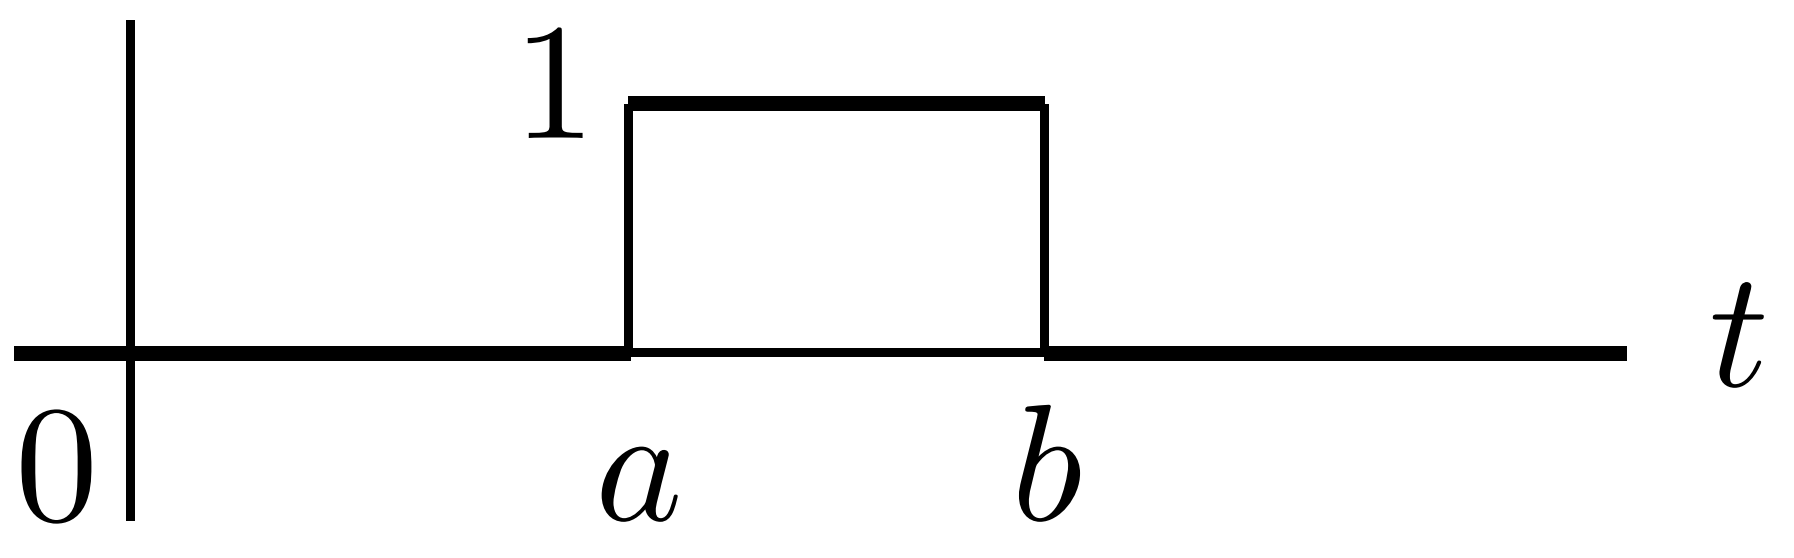
\includegraphics[width=0.25\textwidth]{../Rss/ODE/L25} & \centering \[\frac{e^{-ap}-e^-bp}{p}\] & \[\text{All }p\]\\
            \[\mathcal{L}26\] &\raisebox{-0.75\totalheight}{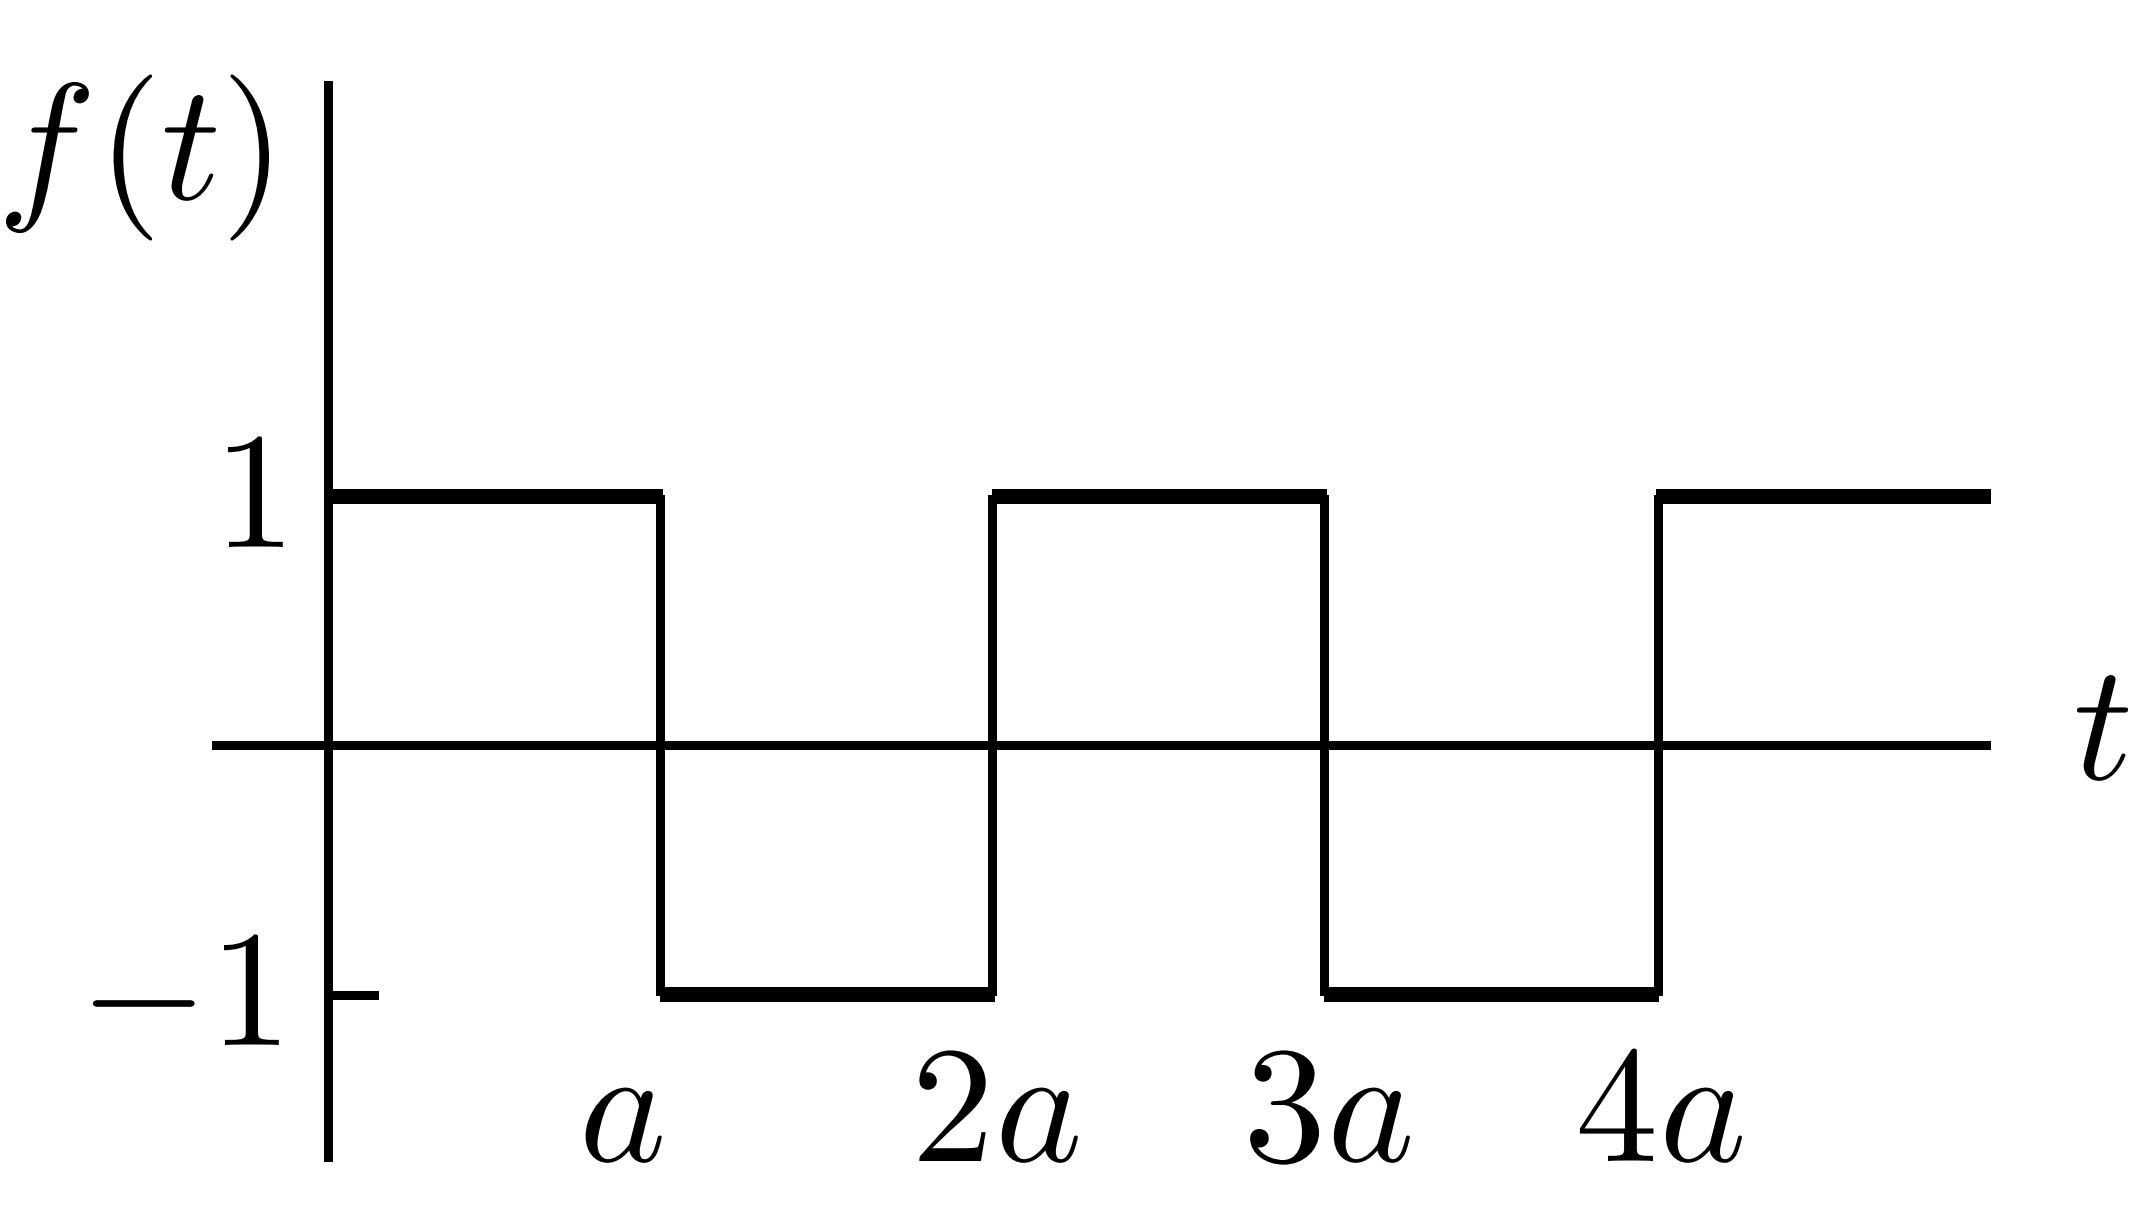
\includegraphics[width=0.25\textwidth]{../Rss/ODE/L26}}& \centering \[\frac{1}{p}\tanh \frac{ap}{2}\] & \[\text{All }p\]\\
        \end{longtable}
        \begin{longtable}{m{0.05\textwidth}m{0.3\textwidth}  m{0.3\textwidth}m{0.2\textwidth}|}
            \[\mathcal{L}27\] & \multicolumn{1}{p{0.4cm}}{\centering \[ \delta(t-a),a\geq0\]} & \multicolumn{1}{p{0.4cm}}{\centering \[e^{-pa}\]}\\
            \vspace*{0.1cm} 
        \[\mathcal{L}28\] &\multicolumn{1}{p{0.4\textwidth}}{\centering {\begin{align*}f(t)&=\begin{cases}g(t-a), &t>a>0\\0,&t<a \end{cases}\\
            &=g(t-a)u(t-a)\end{align*}}}& \multicolumn{1}{p{0.4\textwidth}}{\centering \[e^{-pa}G(p)\]
        \(G(p)\) means \(\mathcal{L}(g)\). Therefore \(e^{-pa}\mathcal{L}[g(t-a)]\)}\\

        \[\mathcal{L}29\] & \multicolumn{1}{p{0.4\textwidth}}{\centering \[e^{-at}g(t) \]} & \multicolumn{2}{p{0.4\textwidth}}{\centering \[ G(p+a)\]}\\

        \[\mathcal{L}30\] &\multicolumn{1}{p{0.4\textwidth}}{\centering \[ g(at),a>0\]} & \multicolumn{2}{p{0.4\textwidth}}{\centering \[ \frac{1}{a}G\biggl(\frac{p}{a}\biggr)\]}\\

        \vspace*{0.1cm}
        \[\mathcal{L}31\] & \multicolumn{1}{p{0.4\textwidth}}{\centering \[ \frac{g(t)}{t}\]if integrable} & \multicolumn{2}{p{0.4\textwidth}}{\centering \[ \int_{p}^{\infty}G(u)\;du\]}\\

        \[\mathcal{L}32\] & \multicolumn{1}{p{0.4\textwidth}}{\centering {\[t^n g(t) \]}} & \multicolumn{1}{p{0.4\textwidth}}{\centering {\[(-1)^n {\biggl(\frac{d}{dp}\biggr)}^n (G(p))\]}}\\

        \vspace*{-0.15cm}
        \[\mathcal{L}33\] &\multicolumn{1}{p{0.4\textwidth}}{\centering \[\int_{0}^{t }g(\tau)\;d\tau \]} & \multicolumn{2}{p{0.4\textwidth}}{\centering \[ \frac{1}{p}G(p)\]}\\

        \vspace*{0.1cm}
        \[\mathcal{L}34\] & \multicolumn{1}{p{0.4\textwidth}}{\centering Convolution of \(g\) and \(h\), often written as \[g*h\]
        \[ \int_{0}^{t}g(t-\tau)h(\tau)\;d\tau= \int_{0}^{t}g(\tau)h(t-\tau)\;d\tau\]} & \multicolumn{2}{p{0.4\textwidth}}{\centering \[ G(p)H(p)\]}\\
        \end{longtable}
        \begin{longtable}{m{0.05\textwidth}m{0.3\textwidth}  m{0.3\textwidth}m{0.2\textwidth}|}
            \[\mathcal{L}35\] &\multicolumn{3}{p{1\textwidth}}{ Transforms of derivatives of y }\\
        \end{longtable}
        \begin{align*}
            \mathcal{L}(y)&=Y\\
            \mathcal{L}(y') &= pY - y\\
            \mathcal{L}(y'') &= p^2Y -p y_0-y_0'\\
            \mathcal{L}(y''') &= p^3Y -p^2y_0-py_0'-y_0\\
            \mathcal{L}(y^n) &= p^nY -p^{n-1} y_0-p^{n-2}y_0'-\dots-y_0^{n-1}\\
        \end{align*}
\end{document}